\documentclass{article}
\usepackage{import}
\subimport{../}{preamble}
\begin{document}

\section{Plasmon Coupling}

% Basic introduction to charge interaction and gap modes
Both the resonant field enhancement and the confinement of a surface plasmon can be improved by bringing a second plasmon into close proximity. Similar to coupled harmonic oscillators and dipoles, plasmons couple together via Coulomb forces once brought together, forming normal modes of oscillation across interacting charge distributions. In many cases the charge distribution of the resulting normal mode is strongly confined to the dielectric space between metallic surfaces where charges strongly interact. Normal modes are therefore more generally known as \emph{gap plasmons}. It is the existence of gap plasmons that has both enabled single molecule spectroscopy and resulted in the large degree of spectral tuning observed in composite plasmonic systems.

Coupled plasmons are a feature of many metallic nano-systems with closely spaced metal-dielectric interfaces, including \gls{mim} and \gls{imi} waveguides and systems containing multiple \glspl{mnp}. For the purposes of this work, discussion is restricted to the ideal case of coupled \glspl{lsp} between two closely spaced \glspl{mnp}, though the description of coupling is valid for many other cases involving \glspl{sp}.

\subsection{Localised Surface Plasmon Hybridisation in Nano-Gap Cavities}

In the simplest case, only multipolar plasmons, excited in two spherical \glspl{mnp} being driven by external \gls{em} fields, are considered. This is the prototypical plasmonic dimer system used to understand plasmon coupling. Similar systems, including chains of \glspl{mnp} \cite{maier2002} and \glspl{mnp} on mirrors \cite{mertens2013, denijs2014}, have been used to study plasmon coupling. In each of these systems, the physics can be reduced to the interaction between neighbouring charge distributions. This is why the simple dimer system is important to fully understand.

The behaviour of a plasmonic dimer stems from the Coulomb interaction between free electrons in adjacent metallic nanostructures. As \glspl{mnp} move closer together the force between charges grows, increasingly polarising the local gap region to which the charge becomes confined. The introduction of separation-dependent forces to the plasmon oscillator shifts the resonance frequency of the individual plasmon mode from $\omega_0$ by $\Delta\omega$ depending on the strength of coupling. Since coupling is between multipolar fields, the relative orientation between excited \glspl{lsp} and the external driving field is important to determine the sign and strength of coupling. Coupling is strongest when adjacent plasmon poles are oppositely charged. This is generally the case for \glspl{lsp} in a \gls{mnp} dimer being driven in phase with the incident field.

% Field enhancement increase
The primary effect of gap plasmon excitation is the localisation of the electric field to the dielectric gap medium. As stated previously, a plasmon intrinsically enhances the near-field around a \gls{mnp}, caused by optically-driven charge accumulation at the metal-dielectric interface. For the case of two interacting plasmonic particles, the Coulomb forces between plasmons pulls charge more towards the gap region. As a result, a greater amount of charge accumulates on the metal surfaces around the gap and the field in the gap cavity becomes more localised and further enhanced.%
\footnote{This is much like with charged plates in a capacitor and how the field increases with dielectric gap material, spacing and charge accumulation.}
For a strongly confined gap mode there is very little field in the metal with almost all field confined within a small lateral mode within the gap. This is known as a plasmonic ``hot spot". Through this mechanism alone the field enhancement $\left|E/E_0\right|$ can be increased by more than an order of magnitude. For this reason, attention has shifted from individual plasmonic nanostructures to coupled systems to extract the maximum performance.

\begin{figure}[bt]
\centering
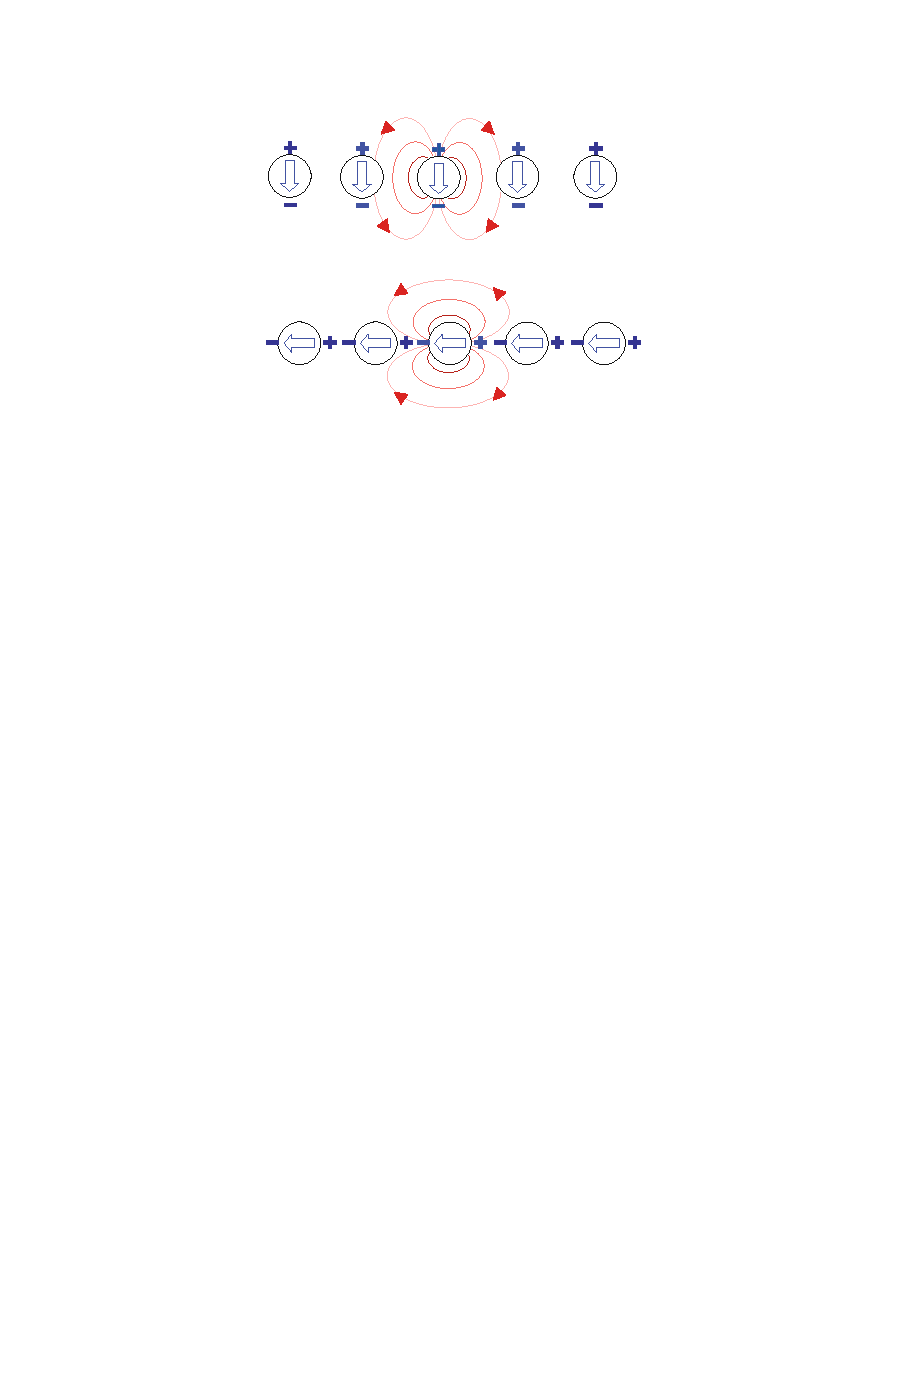
\includegraphics[width=0.45\textwidth]{figures/literature/maier_plasmonics_coupling_diagram}
\quad
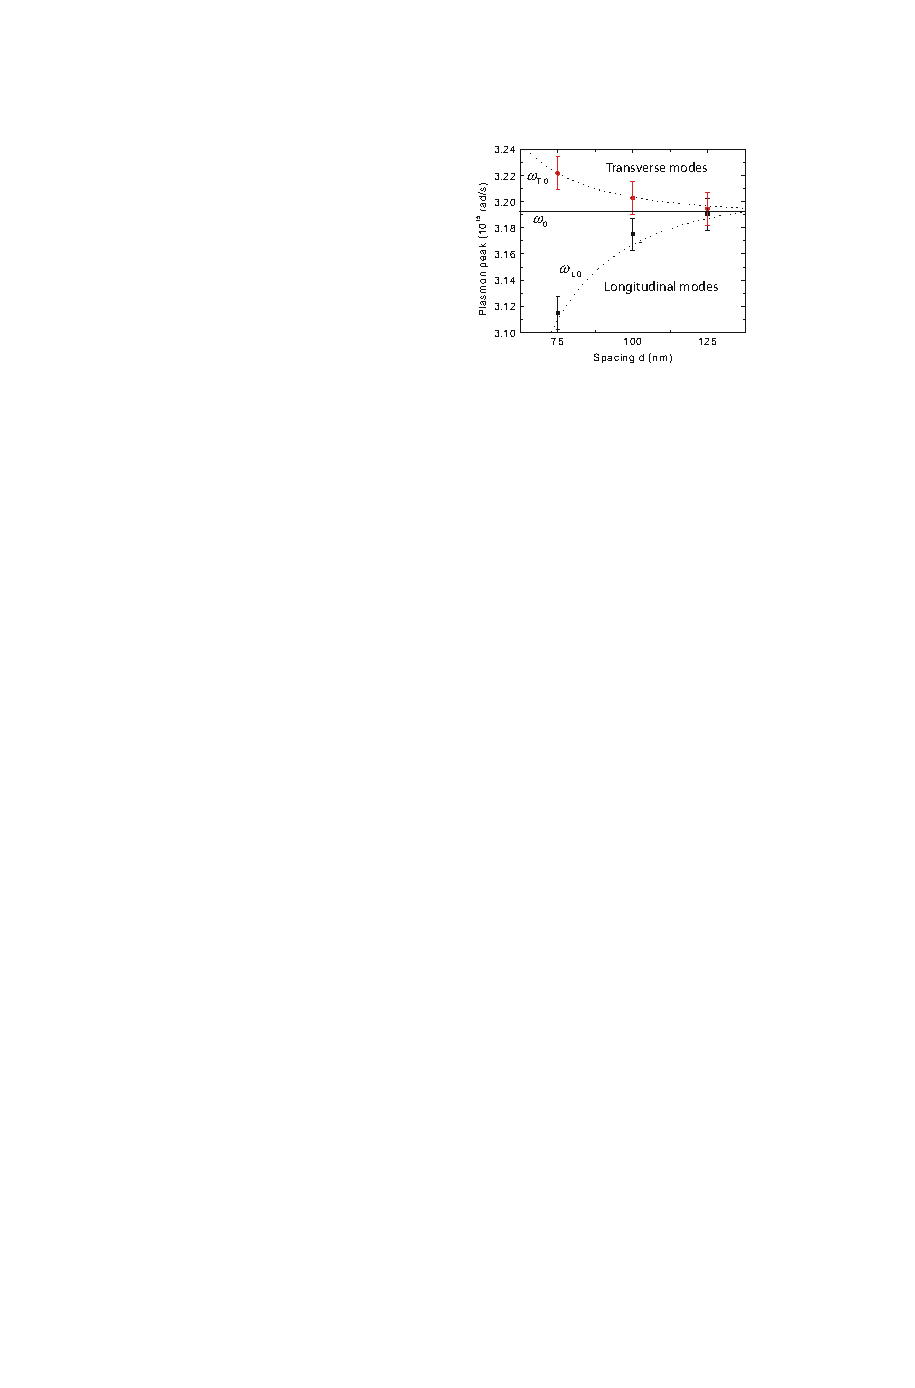
\includegraphics[width=0.45\textwidth]{figures/literature/maier_plasmonics_coupling}
\caption[Experimental and theoretical plasmon coupling]{\textbf{Experimental and theoretical plasmon coupling.} Dipolar plasmons in chains of spherical AuNPs couple depending on field orientation \cite{maier2007plasmonics} (left). Experimentally measured plasmon resonance energies in coupled AuNP chains show the gap-dependent tuning due to coupling \cite{maier2002} (right). The dotted line corresponds to a $r^{-3}$ point dipole model.}
\label{fig:maier_plasmon_coupling}
\end{figure}

% Experimental evidence
Systems of AuNPs were experimentally studied from 2002 \cite{maier2002}, in which the individual resonances of AuNP chains with different spacings were shown to couple and form two new modes gradually separating in energy with increased coupling strength (\figurename~\ref{fig:maier_plasmon_coupling}). These modes are the in-phase coupled modes between particles in orthogonal polarisations. The resonance along the chain redshifts with increased coupling due to attraction between plasmons whereas the resonances perpendicular to the chain blueshift as dipolar plasmons in this orientation repel. % is there anymore evidence for this?

\begin{wrapfigure}{O}{0.35\textwidth}
\vspace{-10pt}
\fontsize{10pt}{1em}\selectfont
\def\svgwidth{\textwidth}
\subimport{./figures/}{dipole_interactions.pdf_tex}
\caption[Diagram of dipole interactions]{\textbf{Diagram of dipole interactions.} Dipoles have length $D$. The distance between dipoles is $r$ with an edge-to-edge separation $d$. Configurations 1 and 3 are comparable with plasmon coupling as a result of sub-wavelength structures being driven by a single external light field. Configurations 2 and 4 are generally unphysical without significantly increasing the system size.}
\label{fig:dipole_interactions}
\vspace{-5pt}
\end{wrapfigure}

Interactions between plasmons appear similar to dipole-dipole interactions, which also depend on separation and relative orientation. Examples of some commonly considered dipole-dipole interaction geometries are shown in \figurename~\ref{fig:dipole_interactions}. For two parallel dipoles aligned along their axes, driven in phase, the attractive coupling potential increases with decreasing separation, $r$, as $V \propto p_1p_2r^{-3}$ \cite{halas2011}. For an oscillating dipole this redshifts (decreases) the resonant frequency. Conversely, the repulsive interaction between two parallel dipoles positioned side by side also increases as $r^{-3}$, but blueshifts (increases) the resonant frequency. Symmetric anti-phase configurations lead to local field cancellation. Observation of such modes only becomes possible in non-symmetric dipole-dipole systems. Alternatively, for dimers outside of the quasistatic regime, phase retardation of the driving field across the dimer is capable of breaking the coupling symmetry, allowing these modes to be excited.

For plasmons in \glspl{mnp}, the coupling interaction is well approximated using the dipole-dipole model \cite{kreibig1995optical, maier2002, gluodenis2002, rechberger2003, atay2004}, however the restoring force within the particles also contributes to the potential and goes as the volume $D^3$. The interaction energy between two plasmons therefore goes as $(r/D)^{-3}$. Since the gap size, $\gls{d}=r-D$, is the defining feature of a plasmonic dimer, relations are often expressed in the quantity $(d/D) = (r/D)-1$ rather than using the centre of mass separation. The resonant wavelength shift due to coupling can then be described using a plasmon ruler equation \cite{jain2007, ben2011},
\begin{equation}
	\frac{\Delta\lambda}{\lambda_0} = a\exp\left(-\frac{(d/D)}{\tau}\right),
	\label{eq:plasmon_ruler}
\end{equation}
where $a$ is the coupling strength and $\tau$ is a decay constant. The exponential decay is considered to be approximately equivalent to the $(d/D)^{-3}$ behaviour, which is expressed in terms of shape and size parameters, $\Lambda$ and $\gamma$, as,
\begin{equation}
	\frac{\Delta\lambda}{\lambda_0} = \frac{1}{12\Lambda(d/D+1)^3 - (1-\gamma)}.
\end{equation}
In recent years this relation still shows good agreement with experimental data but the approach remains limited to describing only dipolar modes in simple geometries. % add citation?

% Plasmon hybridisation theory
\begin{figure}[bt]
\centering
\fontsize{10pt}{1em}\selectfont
\def\svgwidth{0.98\textwidth}
\subimport{./figures/}{plasmon_dimer_hybridisation.pdf_tex}
\caption[Diagram of plasmon hybridisation between coupled plasmons in a nanoparticle dimer]{\textbf{Diagram of plasmon hybridisation between coupled plasmons in a nanoparticle dimer.} Plasmons are coupled along the dimer axis. Coupling leads to bonding and anti-bonding modes for each set of interacting $l$ modes. Interaction with higher order $l$ modes lowers the overall energy of lower order coupled modes (green lines). Only the bonding ($\omega_{\uparrow\uparrow}$) mode in the symmetric (homo-)dimer has a net dipole moment and is therefore observable. Cancellation of the net dipole moment means the anti-bonding ($\omega_{\uparrow\downarrow}$) mode remains optically dark. On the contrary, asymmetry in a (hetero-)dimer means both modes stay bright with the lower and higher energy individual modes forming the bonding and anti-bonding hybridised modes, respectively. This diagram is adapted from \cite{nordlander2004}.}
\label{fig:plasmon_hybridisation}
\end{figure}

A slightly more complex model explaining the formation and behaviour of coupled modes was developed between 2003 and 2004. Plasmon hybridisation describes the plasmon resonances of a complex particle geometry by {\color{red}deconstructing/decomposing} it into two simpler geometries \cite{prodan2003, prodan2004}. This is done in analogy with the ideas underpinning molecular orbital hybridisation and the hybridisation of quantum energy states. Using this logic, the theory equally describes the plasmon resonances of two coupled simple particle geometries \cite{nordlander2004} or a particle coupled with its image charge in a surface \cite{nordlander2004a}. The multipolar modes of the individual dimer particles split in energy into two hybridised modes representing the bonding (in-phase) and anti-bonding (anti-phase) pole configurations. Due to the attractive and repulsive nature of the bonding and anti-bonding configurations the coupled modes redshift and blueshift from the initial mode position with decreasing separation, respectively. This behaviour is shown in \figurename~\ref{fig:plasmon_hybridisation}.

% bonding vs anti-bonding
This model clearly shows that the bonding and anti-bonding modes have very different radiative properties. The bonding dipole exhibits a large net dipole moment due to parallel alignment of individual dipoles, whereas the anti-parallel aligned anti-bonding mode has no net dipole. As a result, the bonding mode strongly couples with light whereas the anti-bonding mode remains dark. Anti-bonding modes are consequently referred to as dark modes in symmetric systems. As stated earlier, should the mode acquire a finite net dipole, either through asymmetry of the dimer particles (difference material, size or shape) or phase retardation, it can become radiative and therefore experimentally observable. If this occurs then two resonances are observed upon coupling. The higher energy resonance blueshifts with decreasing separation to form the anti-bonding mode whilst the lower energy resonance redshifts and forms the bonding mode.

% mixing of different l modes
Hybridisation between two $l=i$ modes is also influenced by the presence of other modes of $l \neq i$, as is shown by the second set of dashed lines in \figurename~\ref{fig:plasmon_hybridisation}. For most simple dimer systems only the $l=1$ mode is observed, however, with small gaps or large particles, higher order modes becomes observable. The $l=1$ mode then experiences an increased rate of redshifting due to interaction with the appearing $l=2$ mode {\color{red}and so on}. Should the gap size become small enough, interaction between the redshifting bonding $l=2$ mode and the blueshifting anti-bonding $l=1$ mode can reverse the blueshift of the anti-bonding mode \cite{nordlander2004}. Classically, for nm-size gaps, a whole range of higher order modes are expected to exist in the gap \cite{romero2006}. The lateral confinement of these modes across the gap is estimated using, % how is this mode dependent?
\begin{equation}
	w = \sqrt{Rd}.
\end{equation}
% polarisation effects
As with dipole coupling, an opposite effect occurs when the driving field is orientation perpendicular to the dimer axis. In this instance the excited plasmon poles repel each other more with decreasing separation and the bonding mode therefore blueshifts \cite{gunnarsson2005, yang2010}.

\subsection{The Dynamical Optical Response of Plasmonic Dimers: Transitioning from Capacitive to Conductive Plasmonic Coupling}
% \cite{kadkhodazadeh2013} should go in last chapter, \cite{elkhoury2014} maybe to include

Using modern numerical simulation techniques, the full separation-dependent optical response of a plasmonic dimer has been calculated as particles transition from non-interacting to hybridisation through to geometrical contact \cite{romero2006}. In these calculations, the lowest order plasmons hybridise, redshift and more intensely scatter as the separation decreases, with higher order modes eventually emerging. As the higher order modes become more intense, scattering from the lower order modes decreases. Despite this, their field enhancement continues to rise. These plasmons becoming so confined that they no longer couple with the far-field. This behaviour continues until the particles touch into geometrical contact.

\begin{figure}[bt]
\centering
\fontsize{10pt}{1em}\selectfont
\def\svgwidth{0.65\textwidth}
\subimport{./figures/}{plasmon_contact.pdf_tex}
\caption[Diagram showing the emergence of charge transfer and screened bonding (crevice) plasmons on geometrical contact in a nanoparticle dimer]{\textbf{Diagram showing the emergence of charge transfer and screened bonding (crevice) plasmons on geometrical contact in a nanoparticle dimer.} The field generated by the bonding dimer plasmon (BDP) is screened from the gap by the conductive contact, forcing capacitive coupling to the crevice gap in the form of the screened bonding dimer plasmon (SBDP). The dominant charge oscillation is then the charge transfer plasmon (CTP) through the conductive bridge and across the whole structure.}
\label{fig:plasmon_contact}
\end{figure}

Once in geometrical contact the gap becomes a conductive bridge. If it's length is small and it's conductance large, such that charge can be transported between particles within half an optical cycle, then \glspl{ctp} can form. The conductive short prevents the accumulation of surface charge on gap-facing metallic interfaces, reducing the capacitive coupling between plasmons (\figurename~\ref{fig:plasmon_contact}). The bonding hybridised coupled modes are screened and forced outwards towards the crevice \cite{romero2006, perez2010, tserkezis2014}. In another sense there are a finite number of electrons, each in a specific state, therefore if one electron transitions into a collective \gls{ctp} oscillation then it's contribution is lost from it's original capacitive mode.

\gls{ctp} modes, with their spatially larger dipoles, form at lower energies than the bonding modes upon geometrical contact. As particles overlap, the dipole length decreases, increasing it's energy, and \glspl{ctp} resonances blueshift \cite{romero2006}. Each bonding mode has an associated \gls{ctp} mode, corresponding to the screening and broadening of that mode's capacitive interaction since the gap conductivity $\sigma$ and the local dielectric function \dielectric\ are related.%
\footnote{For a spherical \gls{mnp} dimer with bonding hybridised dipolar (BDP) and quadrupolar (BQP) modes the corresponding CTP modes are typically labelled as CTP and CTP$^\prime$.}
Greater overlap between particles widens the junction and increases the conductance, which, along with geometrical changes, strongly modifies the plasmonics. By lithographically creating overlapping discs it has been shown that the modes blueshift back to the single particle resonance upon complete overlap \cite{atay2004, lassiter2008}.

% Screening effect
The previously described effects can be broken down into a function of the contact geometry in the gap, where the gap between particles of radius $R$ has a width $d$, conductivity $\sigma$ with a conductive linker of radius $a$. Depending on these parameters there are two effects of a conductive linker - capacitive screening and charge transfer \cite{perez2010}. Screening occurs at low conductances once a contact has formed whereas excitation of a \gls{ctp} requires a higher junction conductance. The conductance threshold for screening of the dipolar bonding plasmon is given by,
\begin{equation}
	G_{\mathrm{SBDP}} = \frac{\omega_{\mathrm{BDP}}}{2\pi}\frac{a^2}{d}.
\end{equation}
The threshold is intrinsically independent of geometry and depends only on the conductivity ($\sigma_{\mathrm{SBDP}} = \omega_{\mathrm{BDP}}/2\pi^2$). For larger contact widths or shorter linker lengths the threshold increases to overcome the increased capacitive coupling.
% CTP effect
A second threshold exists for \gls{ctp} formation, occurring at,
\begin{equation}
	G_{\mathrm{CTP}} = \frac{\omega_{\mathrm{CTP}}}{4\pi}\frac{R^2}{d}.
\end{equation}
Similarly to $G_{\mathrm{SBDP}}$, the conductivity threshold is expressed as $\sigma_{\mathrm{CTP}} = (\omega_{\mathrm{CTP}}/4\pi^2) (R/a)^2$. Unlike screening, \gls{ctp} formation depends not only on the conductivity but the junction geometry. The geometry factor $(R/a)$ represents the ratio between the total charge in the particle and the amount which can pass through a gap with fixed conductivity. Having a large conductivity means the junction does not have to be as wide, relative to the particle size, to accommodate enough current to maintain a \gls{ctp}.

These results can be better understood in a number of limiting cases. For a fixed linked dimer geometry the optics can be controlled through the gap conductivity. Increasing the conductivity leads to screening, and therefore blueshifting, of the bonding mode before a \gls{ctp} emerges \cite{perez2011, zabala2011}. Since the geometry does not change the \gls{ctp}, once excited, does not tune and the blueshift of the screened mode saturates. These systems have been experimentally realised using fractional mixing of conductive and insulating \glspl{sam}, with results suggesting a 1\G0 threshold to observe screening \cite{benz2014}. In the event that the linker originates from the dimer metal, i.e. a AuNP dimer linked by a Au constriction, then the conductivity remains fixed and the width of the contact determines the extent of charge transfer. Under these conditions, screening occurs as expected and the \gls{ctp} energy increases with linker width \cite{perez2011}. \Glspl{mnp} dimers fixed by hollow spacer molecules have exhibited this effect after high power laser pulses create Au threads of various widths \cite{herrmann2014, tserkezis2014}. Dimers in which the gap width changes, leading to overlap, form the more complex system to understand since the geometrical changes also influence the plasmonics along with charge transfer.

This summarises the classical picture of plasmon coupling from capacitive to conductive coupling. However, the predictions of hybridisation theory break down at small, sub-nm gaps. Classical theory suggests that a continuum of higher order modes will be excited and redshift to a singularity as $d \rightarrow 0$, with the field enhancement increasing infinitely. This is completely unphysical behaviour and is rectified when quantum mechanics is considered.
% Onset of tunnelling
The classical picture description breaks down under two conditions - either the particles become sufficiently small that quantum non-locality and non-local effects (finite, non-negligible electron wavefunction spill-out from the particle) become important or the gap size decreases to scales on which quantum tunnelling can no longer be ignored. The onset of quantum tunnelling means charge is transported across the gap without requiring geometrical contact, rectifying the singularity predicted by classical electromagnetism.

\begin{figure}[bt]
\centering
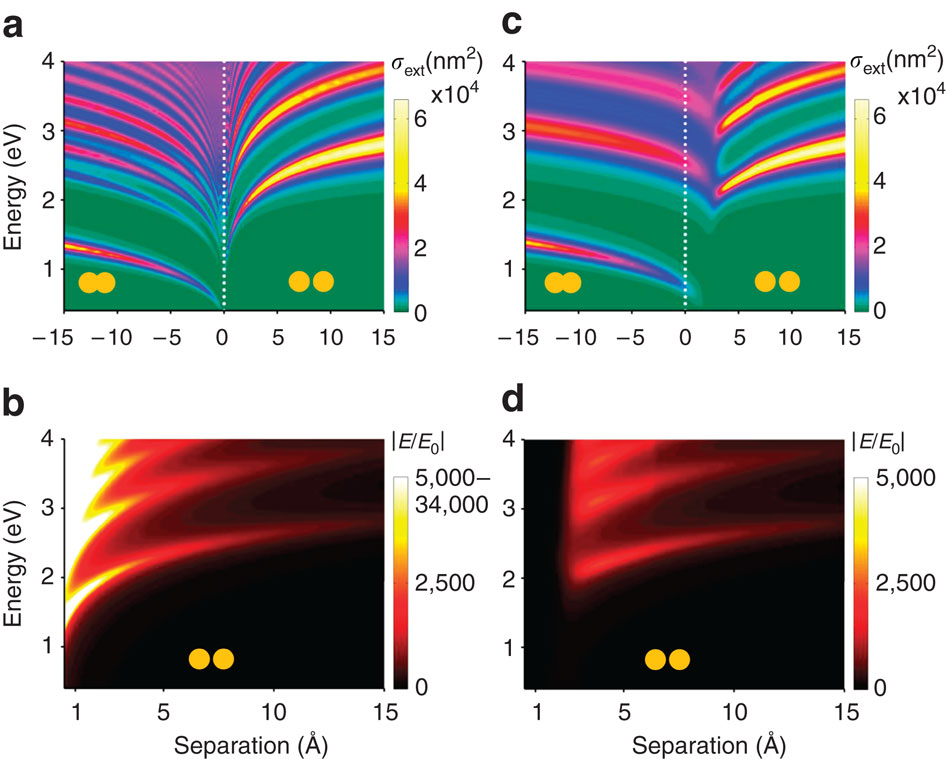
\includegraphics[width=0.7\textwidth]{figures/literature/ncomms1806-f4}
\caption[Numerical calculated extinction cross-section and field enhancement of a spherical AuNP dimer as a function of gap separation \cite{esteban2012}]{\textbf{Numerical calculated extinction cross-section and field enhancement of a spherical AuNP dimer as a function of gap separation \cite{esteban2012}.} The classical approach (left), valid for separations greater than $\sim$\SI{5}{\angstrom}, shows many modes redshifting into a singularity on geometrical contact, following by blueshifting CTP modes as the particles overlap. Introduction of an effective (conductive) gap medium to emulate the effects of quantum tunnelling (quantum corrected model, right) demonstrate the early onset of screening and CTP formation prior to geometrical contact. Figure taken from \cite{esteban2012}.}
\label{fig:optical_response_dimer}
\end{figure}

The effects of quantum tunnelling were first predicted in small ($R<\SI{2}{nm}$) Na\glspl{np} using full quantum mechanical, time-dependent \gls{dft} calculations \cite{zuloaga2009}. Since these calculations consider the behaviour of each electron, they are limited in complexity to small systems containing less than 2000 electrons. Tunnelling effects in larger metallic nanostructures are predicted by the \gls{qcm}, a classical model which uses an effective gap dielectric function that takes into account the conductivity induced by quantum effects using pre-calculated values from \gls{dft} \cite{esteban2012}. For large surfaces and small gaps the integrated contribution to conductance from tunnelling across the gap is enough to initially screen the bonding plasmons followed by the formation of \glspl{ctp} (\figurename~\ref{fig:optical_response_dimer}). Screening leads to strong attenuation of the field enhancement in the gap. The lack of modes present when considering quantum effects is a result of electron tunnelling smoothing the effective junction surface. {\color{red}Additionally, whilst the bonding mode appears to blueshift as a result of screening, simulations suggest that the blueshifting resonance is a higher order \gls{ctp} excitation.}

\begin{figure}[bt]
\centering
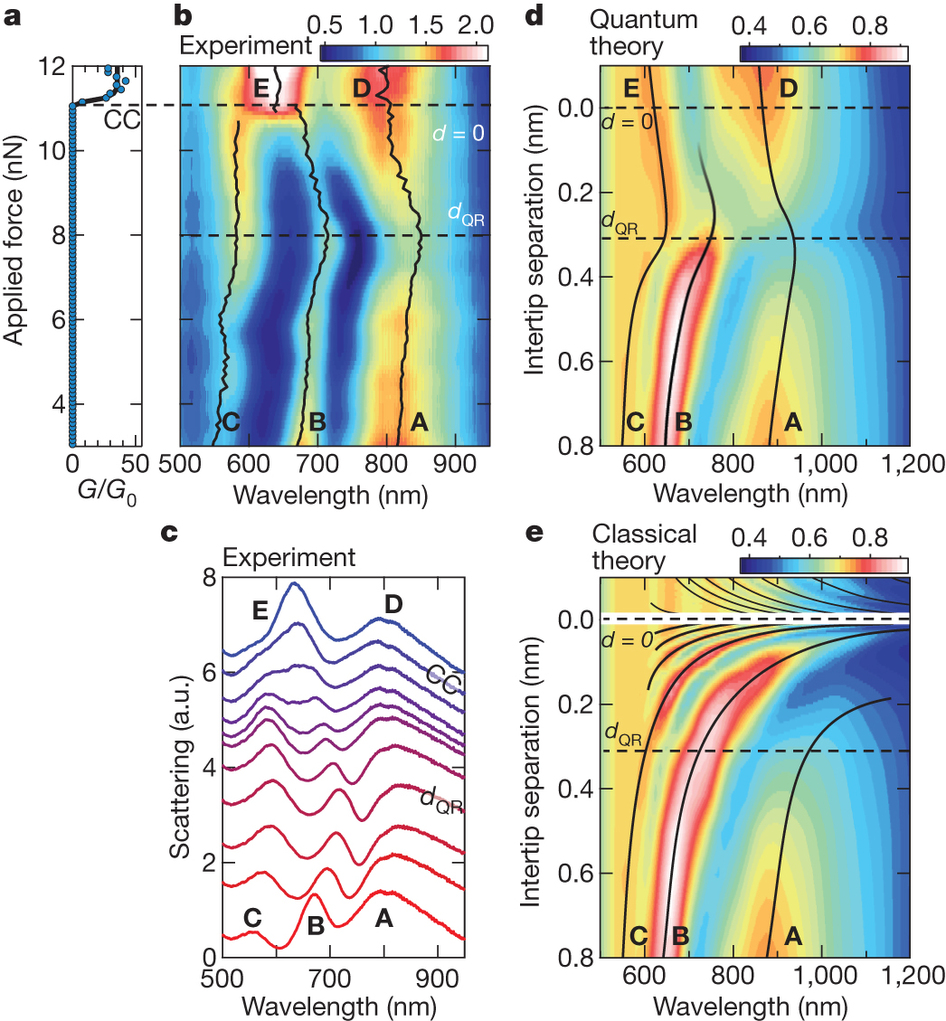
\includegraphics[width=0.65\textwidth, clip=true, trim=0 500 0 0]{figures/literature/nature11653-f2_2}\\
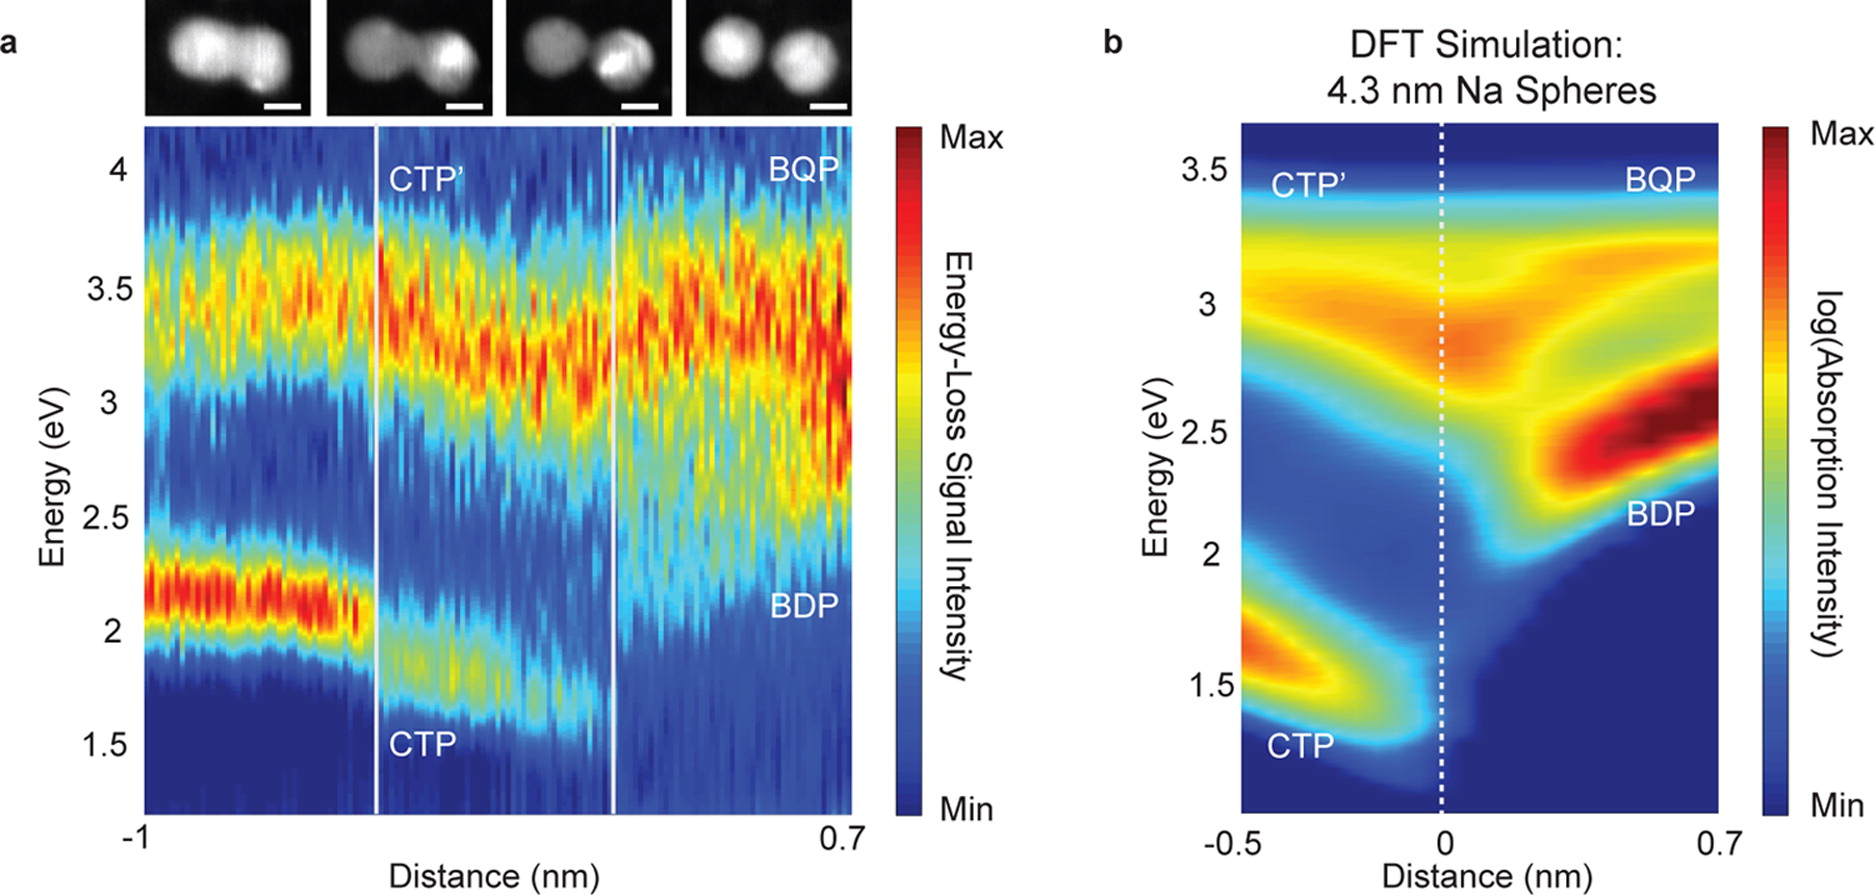
\includegraphics[width=0.65\textwidth]{figures/literature/nl-2012-04078v_0001}
\caption[Examples of experimental measurements of the effect of quantum tunnelling on plasmonic gap systems]{\textbf{Examples of experimental measurements of the effect of quantum tunnelling on plasmonic gap systems through direct monitoring of the plasmon resonances.} (top) Supercontinuum dark-field scattering measurements of two \SI{300}{nm} diameter spherical Au tips in a dimer configuration with reducing separation, transitioning below \SI{1}{nm} and into the quantum regime \cite{savage2012}. (bottom) EELS measurements of \SI{10}{nm} AgNPs being induced closer together by the electron beam \cite{scholl2013}.}
\label{fig:tunnelling_plasmonics}
\end{figure}

% Experimental measurements
Experimental evidence of quantum tunnelling influencing plasmon coupling has been observed using both optical spectroscopy \cite{savage2012, cha2014, zhu2014}, \gls{eels} \cite{scholl2013}, \gls{sers} \cite{zhu2014}, photoluminescence \cite{kravtsov2014} and third-harmonic generation measurements \cite{hajisalem2014}.
% Direct measurements
First measurements were made using optical scattering from a dynamic spherically-tipped Au AFM probe dimer, with simulated spectra using the \gls{qcm} (\figurename~\ref{fig:tunnelling_plasmonics}) \cite{savage2012}. Plasmon modes are shown to blueshift upon decreasing past a critical separation. Scattering spectra qualitatively agreed with the \gls{qcm}, with discrepancies attributed to difficulty in simulating an extended dual tip geometry. Better agreement with \gls{dft} calculations was found in \gls{eels} measurements on simpler \SI{10}{nm} AgNP dimers, brought together under the influence of the electron beam (\figurename~\ref{fig:tunnelling_plasmonics}) \cite{scholl2013}.
% Molecular distance tuning - note this is not the best quality data or papers
Alkanedithiol molecules of various lengths have also been used to discretely tune the gap separation of AuNP dimers \cite{cha2014}. In this case, blueshifting and attenuation of the bonding dipolar plasmon, as well as an increase in its width, is measured with molecules smaller than pentanedithiol. Similar results are found when using intercalating \glspl{sam} \cite{tan2014}.
% Inferred measurements
Further investigation into sub-nm plasmonic gaps have also shown changes attributed to quantum tunnelling, though inferred from properties depending on the gap field enhancement as opposed to direct measurement of the plasmon resonances. A decrease in signal intensity in both the \gls{sers} peaks \cite{zhu2014} and photoluminescence \cite{kravtsov2014} are signatures of quantum tunnelling screening the coupled plasmon field.

\begin{figure}[bt]
\centering
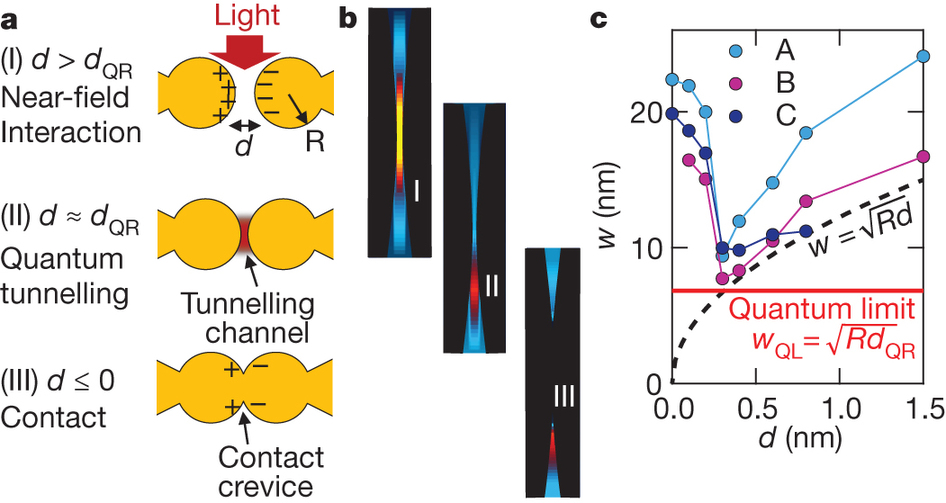
\includegraphics[width=0.6\textwidth]{figures/literature/nature11653-f3_2}
\caption[Plasmon mode distributions in the quantum regime]{\textbf{Plasmon mode distributions in the quantum regime.} Diagram showing the different regimes of plasmonic interaction, taken from \cite{savage2012}. The onset of a tunnelling current pinches of the electric field in the gap via screening/conductive losses prior to conductive contact, which shows a similar expulsion of field from the gap.}
\label{fig:savage2012c}
\end{figure}

Interestingly, qualitative (and to some extent quantitative) agreement between \gls{qcm} calculations and full quantum calculations suggest that the quantum nature of the system is of little importance. Despite only using a classical, resistive gap with conductances given by values characteristic of electron tunnelling, the effects of electron tunnelling on gap plasmons are accurately replicated. This implies that, despite the quantum nature of electron tunnelling, its effects on plasmon coupling depend only on the amount of charge transfer and not the mechanism by which it occurs. This links together work done using particle positioning \cite{savage2012, scholl2013} with studies of interacting plasmonic system coupled with molecular linkers \cite{tan2014, cha2014, benz2014}. Quantum tunnelling still remains an interesting case, however, since it is a form of conduction that is unavoidable once system sizes decrease below \SI{0.5}{nm}. This is why its pinch-off point, the point at which the electric field in the gap is expelled, is described as the quantum limit to plasmon confinement \cite{savage2012}. It is for this reason why it is important to fully understand the relations between plasmonic hot spots and sites of (quantum) charge transfer.

\end{document}